\subsection{UC3 - Modifica di Metadati}
\label{sub:uc2}

\begin{figure}[h]
    \centering
    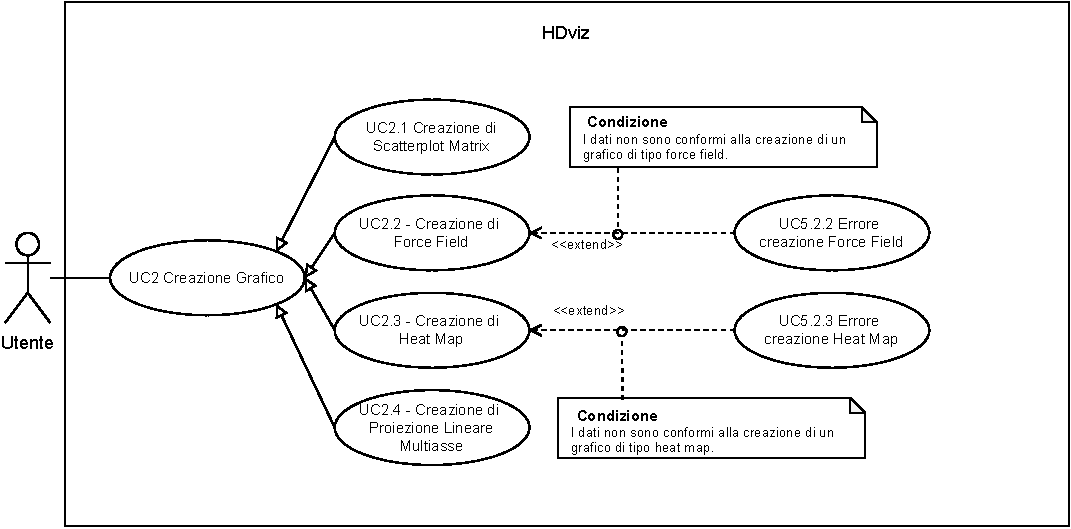
\includegraphics[width=0.5\textwidth]{componenti/casi-duso/diagrammi/UC2.pdf}
    \caption{Diagramma rappresentante UC3}
    \label{fig:UC2}
\end{figure}

\begin{itemize}
    \item \textbf{Descrizione}: Si vogliono modificare i metatag di un dataset già provvisto 
                                di validi metadati.
	
    \item \textbf{Attore primario}: Utente;
    
    \item \textbf{Precondizione}: 	Dei dati sono stati correttamente importati e 
                                    sono associati a dei validi metatag.

	\item \textbf{Postcondizione}:  Ai dati sono stati assegnati dei metatag assegnati dall'utente 

	\item \textbf{Scenario principale}:
		\begin{enumerate}
			\item L'utente seleziona l'opzione di aggiunta modifica dei metatag;
			\item L'utente modifica i metadati degli header che preferisce con metatag validi;
		\end{enumerate}
\end{itemize}

